\documentclass[a4paper,11pt]{report}
\usepackage{chuan_math_gkt}
\usetikzlibrary{angles,quotes,intersections,patterns,decorations.pathreplacing}
\chuanexamsetup

\begin{document}
\examfontsize

\examsecret{绝密$\bigstar$启用前}

\examtitle{2025年普通高等学校招生全国统一考试（北京卷）}{数\quad 学}

\noticetitle
\begin{examnotice}
\item 答卷前，考生务必将自己的姓名、准考证号填写在答题卡上。
\item 回答选择题时，选出每小题的答案后，用铅笔把答题卡上对应题目的答案标号涂黑。如需改动，用橡皮擦干净后，再选涂其他答案标号。回答非选择题时，将答案写在答题卡上。写在本试卷上无效。
\item 考试结束后，将本试卷和答题卡一并交回。
\end{examnotice}


\examsection{一、选择题：本题共10小题，每小题4分，共40分。在每小题给出的四个选项中，只有一项是符合题目要求的。}
\begin{examquestions}
\item 已知集合 $M=\{x\mid 2x-1>5\}$，$N=\{1,2,3\}$，则 $M\cap N=$
\fourchoices{$\{1,2,3\}$}{$\{2,3\}$}{$\{3\}$}{$\varnothing$}
\item 已知复数 $z$ 满足 $\mathrm{i}z+2=2\mathrm{i}$，则 $|z|=$
\fourchoices{$\sqrt2$}{$2\sqrt2$}{$4$}{$8$}
\item 双曲线 $x^2-4y^2=4$ 的离心率为
\fourchoices{\tallchoice{$\dfrac{\sqrt3}{2}$}}{$\dfrac{\sqrt5}{2}$}{$\dfrac54$}{$\sqrt5$}
\item 为了得到函数 $y=9^x$ 的图象，只需把函数 $y=3^x$ 的图象上所有点的
\onechoices{横坐标变为原来的 $\dfrac12$ 倍（纵坐标不变）}{横坐标变为原来的 $2$ 倍（纵坐标不变）}{纵坐标变为原来的 $\dfrac13$ 倍（横坐标不变）}{纵坐标变为原来的 $3$ 倍（横坐标不变）}
\item 已知 $\{a_n\}$ 是公差不为零的等差数列，$a_1=-2$，若 $a_3,a_4,a_6$ 成等比数列，则 $a_{10}=$
\fourchoices{$-20$}{$-18$}{$16$}{$18$}
\item 已知 $a>0,b>0$，则
\twochoices{$a^2+b^2>2ab$}{\tallchoice{$\dfrac1a+\dfrac1b\geq\dfrac1{ab}$}}{\tallchoice{$a+b>\sqrt{ab}$}}{$\dfrac1a+\dfrac1b\leq\dfrac2{\sqrt{ab}}$}
\item 已知函数 $f(x)$ 的定义域为 $D$，则“$f(x)$ 的值域为 $\mathbb R$”是“对任意 $M\in\mathbb R$，存在 $x_0\in D$，使得 $|f(x_0)|>M$”的
\twochoices{充分不必要条件}{必要不充分条件}{充要条件}{既不充分也不必要条件}
\item 设函数 $f(x)=\sin\omega x+\cos\omega x(\omega>0)$，若 $f(x+\pi)=f(x)$ 恒成立，且 $f(x)$ 在 $\left[0,\dfrac\pi4\right]$ 上存在零点，则 $\omega$ 的最小值为
\fourchoices{$8$}{$6$}{$4$}{$3$}
\item 一定条件下，某人工智能大语言模型训练 $N$ 个单位的数据量所需要的时间 $T=k\log_2N$（单位：$\mathrm h$），其中 $k$ 为常数. 在此条件下，已知训练数据量 $N$ 从 $10^6$ 个单位增加到 $1.024\times10^9$ 个单位时，训练时间增加 $20\mathrm h$；当训练数据量 $N$ 从 $1.024\times10^9$ 个单位增加到 $4.096\times10^9$ 个单位时，训练时间增加
\fourchoices{$2\mathrm h$}{$4\mathrm h$}{$20\mathrm h$}{$40\mathrm h$}
\item 在平面直角坐标系 $xOy$ 中，$|\vec{OA}|=|\vec{OB}|=\sqrt2$，$|\vec{AB}|=2$. 设 $C(3,4)$，则 $|2\vec{CA}+\vec{AB}|$ 的取值范围是
\fourchoices{$[6,14]$}{$[6,12]$}{$[8,14]$}{$[8,12]$}
\end{examquestions}

\examsection{二、填空题：本题共5小题，每小题5分，共25分。}
\begin{examquestions}[start=11]
\item 已知抛物线 $y^2=2px(p>0)$ 的顶点到焦点的距离为 $3$，则 $p=$\blank.
\item 已知 $(1-2x)^4=a_0-2a_1x+4a_2x^2-8a_3x^3+16a_4x^4$，则 $a_0=$\blank；$a_1+a_2+a_3+a_4=$\blank.
\item 已知 $\alpha,\beta\in[0,2\pi]$，且 $\sin(\alpha+\beta)=\sin(\alpha-\beta)$，$\cos(\alpha+\beta)\ne\cos(\alpha-\beta)$. 写出满足条件的一组 $\alpha,\beta$ 的值 $\alpha=$\blank，$\beta=$\blank.

\noindent\begin{minipage}[t]{0.62\linewidth}
\item 某科技兴趣小组用 $3D$ 打印机制作的一个零件可以抽象为如图所示的多面体，其中 $ABCDEF$ 是一个平面多边形，平面 $AFR\perp$ 平面 $ABC$，平面 $CDT\perp$ 平面 $ABC$，$AB\perp BC$，$AB\parallel EF\parallel RS\parallel CD$，$BC\parallel DE\parallel ST\parallel AF$. 若 $AB=BC=8$，$AF=CD=4$，$RA=RF=TC=TD=\dfrac52$，则该多面体的体积为\blank.
\end{minipage}\hfill
\begin{minipage}[t]{0.34\linewidth}
\vspace{0em}\centering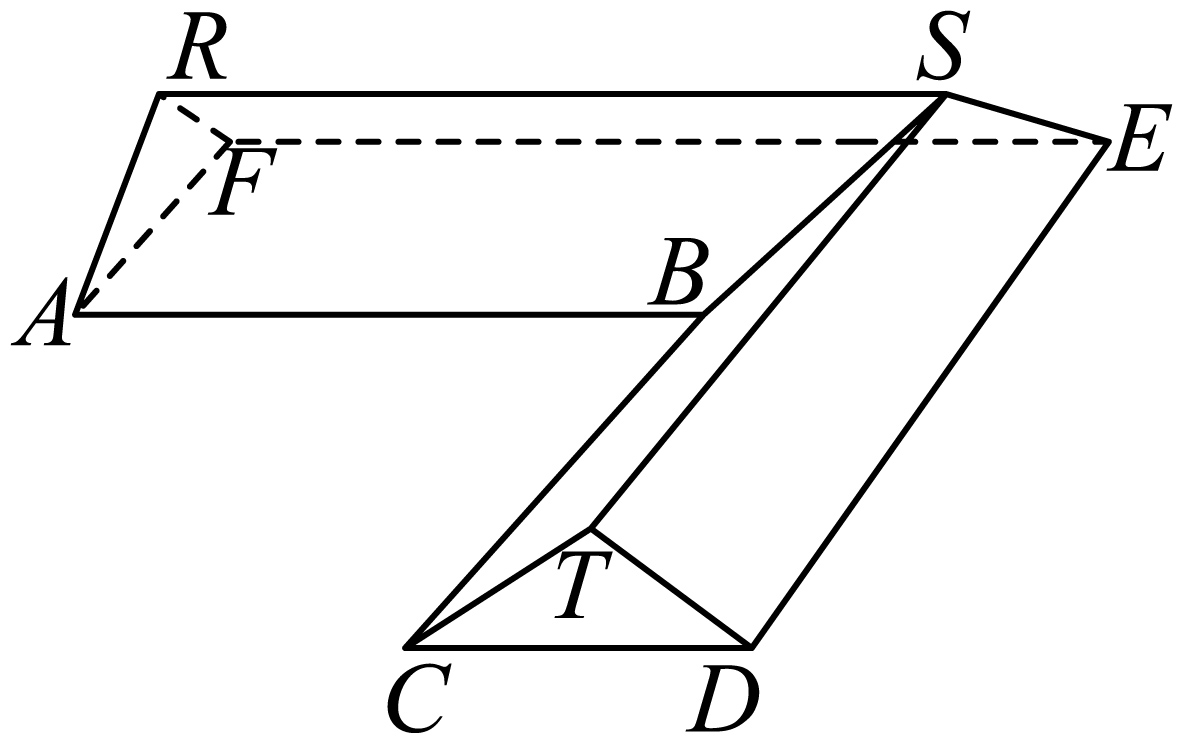
\includegraphics[width=\linewidth]{figures/2025_bj_q14.png}
\end{minipage}

\item 关于定义域为 $\mathbb R$ 的函数 $f(x)$，给出下列四个结论：①存在在 $\mathbb R$ 上单调递增的函数 $f(x)$ 使得 $f(x)+f(2x)=-x$ 恒成立；②存在在 $\mathbb R$ 上单调递减的函数 $f(x)$ 使得 $f(x)-f(2x)=x$ 恒成立；③使得 $f(x)+f(-x)=\cos x$ 恒成立的函数 $f(x)$ 存在且有无穷多个；④使得 $f(x)-f(-x)=\cos x$ 恒成立的函数 $f(x)$ 存在且有无穷多个. 其中正确结论的序号是\blank.
\end{examquestions}

\examsection{三、解答题：本题共6小题，共85分。解答应写出文字说明、证明过程或演算步骤。}
\begin{examanswers}[start=16]
\item（13分）

在 $\triangle ABC$ 中，$\cos A=-\dfrac13$，$a\sin C=4\sqrt2$.

（1）求 $c$ 的值；

（2）再从条件①、条件②、条件③这三个条件中选择一个作为已知，使得 $\triangle ABC$ 存在，求 $BC$ 边上的高.

条件①：$a=6$；条件②：$a\sin B=\dfrac{10\sqrt2}{3}$；条件③：$\triangle ABC$ 面积为 $10\sqrt2$.
\item（13分）

如图，在四棱锥 $P-ABCD$ 中，$\triangle ADC$ 与 $\triangle BAC$ 均为等腰直角三角形，$\angle ADC=90^\circ$，$\angle BAC=90^\circ$，$E$ 为 $BC$ 的中点.

\noindent\begin{minipage}[t]{0.62\linewidth}
（1）若 $F,G$ 分别为 $PD,PE$ 的中点，求证：$FG\parallel$ 平面 $PAB$；

（2）若 $PA\perp$ 平面 $ABCD$，$PA=AC$，求直线 $AB$ 与平面 $PCD$ 所成角的正弦值.
\end{minipage}\hfill
\begin{minipage}[t]{0.30\linewidth}
\vspace{-1em}\centering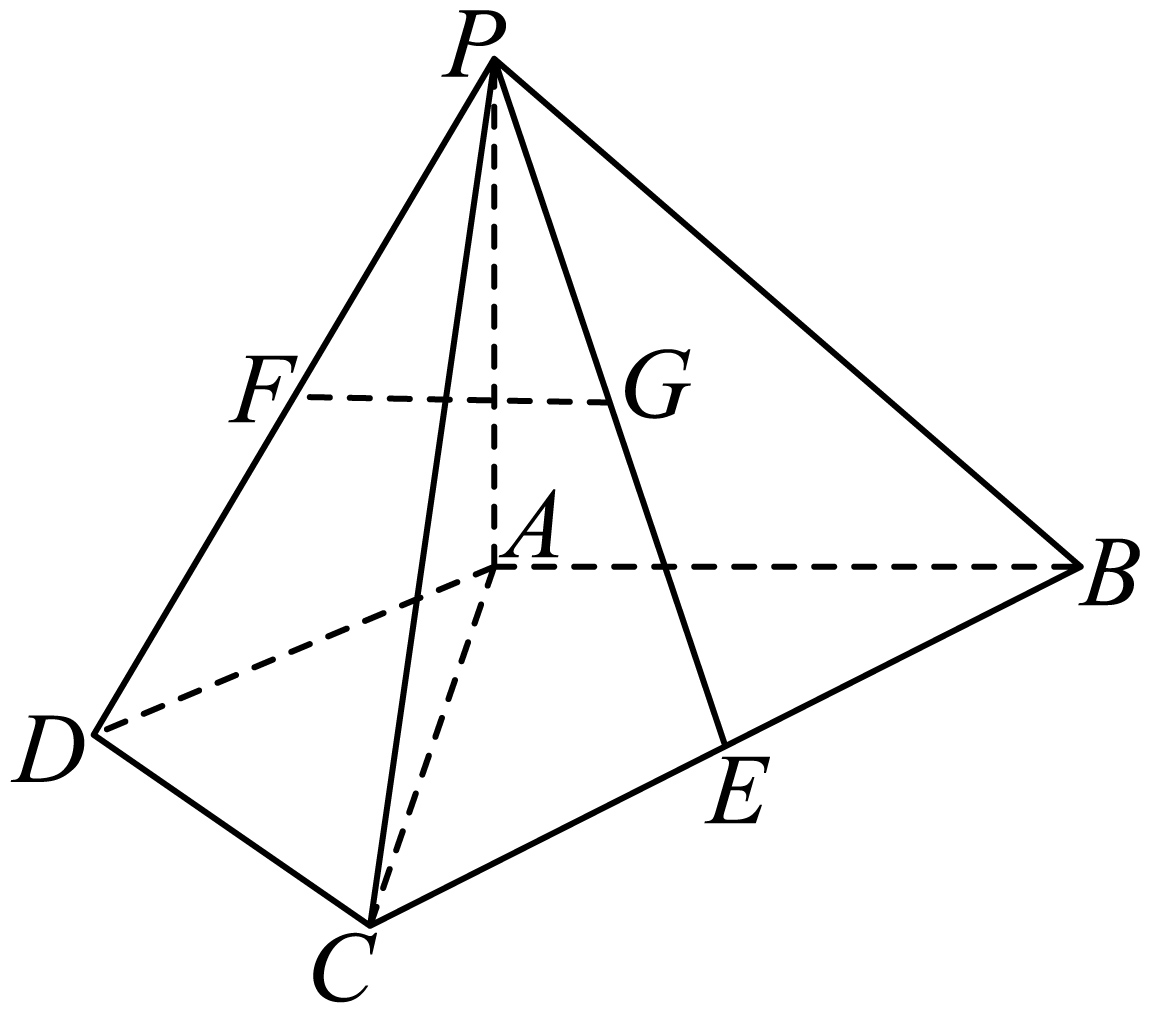
\includegraphics[width=\linewidth]{figures/2025_bj_q17.png}
\end{minipage}
\item（14分）

某次考试中，只有一道单项选择题考查了某个知识点，甲、乙两校的高一年级学生都参加了这次考试. 为了了解学生对该知识点的掌握情况，随机抽查了甲、乙两校高一年级各 $100$ 名学生该题的答题数据，其中甲校学生选择正确的人数为 $80$，乙校学生选择正确的人数为 $75$. 假设学生之间答题相互独立，用频率估计概率.

（1）估计甲校高一年级学生该题选择正确的概率 $p$；

（2）从甲、乙两校高一年级学生中各随机抽取 $1$ 名，设 $X$ 为这 $2$ 名学生中该题选择正确的人数，估计 $X=1$ 的概率及 $X$ 的数学期望；

（3）假设：如果没有掌握该知识点，学生就从题目给出的四个选项中随机选择一个作为答案；如果掌握该知识点，甲校学生选择正确的概率为 $100\%$，乙校学生选择正确的概率为 $85\%$. 设甲、乙两校高一年级学生掌握该知识点的概率估计值分别为 $p_1,p_2$，判断 $p_1$ 与 $p_2$ 的大小（结论不要求证明）.
\item（15分）

已知椭圆 $E:\dfrac{x^2}{a^2}+\dfrac{y^2}{b^2}=1(a>b>0)$ 的离心率为 $\dfrac{\sqrt2}{2}$，椭圆 $E$ 上的点到两焦点的距离之和为 $4$.

（1）求椭圆 $E$ 的方程；

（2）设 $O$ 为坐标原点，点 $M(x_0,y_0)(x_0\ne0)$ 在椭圆 $E$ 上，直线 $x_0x+2y_0y-4=0$ 与直线 $y=2$，$y=-2$ 分别交于点 $A,B$. 设 $\triangle OAM$ 与 $\triangle OBM$ 的面积分别为 $S_1,S_2$，比较 $\dfrac{S_1}{S_2}$ 与 $\dfrac{|OA|}{|OB|}$ 的大小.
\item（15分）

已知函数 $f(x)$ 的定义域是 $(-1,+\infty)$，$f(0)=0$，导函数 $f'(x)=\dfrac{\ln(1+x)}{1+x}$，设 $l_1$ 是曲线 $y=f(x)$ 在点 $A(a,f(a))(a\ne0)$ 处的切线.

（1）求 $f'(x)$ 的最大值；

（2）当 $-1<a<0$ 时，证明：除切点 $A$ 外，曲线 $y=f(x)$ 在直线 $l_1$ 上方；

（3）设过点 $A$ 的直线 $l_2$ 与直线 $l_1$ 垂直，$l_1,l_2$ 与 $x$ 轴交点的横坐标分别是 $x_1,x_2$，若 $a>0$，求 $\dfrac{2a-x_2-x_1}{x_2-x_1}$ 的取值范围.
\item（15分）

已知集合 $A=\{1,2,3,4,5,6,7,8\}$，$M=\{(x,y)\mid x\in A,y\in A\}$，从 $M$ 中选取 $n$ 个不同的元素组成一个序列：$(x_1,y_1),(x_2,y_2),\cdots,(x_n,y_n)$，其中 $(x_i,y_i)$ 称为该序列的第 $i$ 项 $(i=1,2,\cdots,n)$. 若该序列的相邻项 $(x_i,y_i),(x_{i+1},y_{i+1})$ 满足：$\linsys{|x_{i+1}-x_i|=3,\\|y_{i+1}-y_i|=4}$ 或 $\linsys{|x_{i+1}-x_i|=4,\\|y_{i+1}-y_i|=3}$，$(i=1,2,\cdots,n-1)$，则称该序列为 K 列.

（1）对于第 $1$ 项为 $(3,3)$ 的 K 列，写出它的第 $2$ 项；

（2）设 $\Gamma$ 为 K 列，且 $\Gamma$ 中项 $(x_i,y_i)(i=1,2,\cdots,n)$ 满足：当 $i$ 为奇数时，$x_i\in\{1,2,7,8\}$；当 $i$ 为偶数时，$x_i\in\{3,4,5,6\}$. 判断 $(3,2),(4,4)$ 能否同时为 $\Gamma$ 中的项，并说明理由；

（3）证明：由 $M$ 的全部元素组成的序列都不是 K 列.
\end{examanswers}

\end{document}
